\documentclass[10pt,letterpaper]{article}
\usepackage{multicol}
\usepackage{calc}
\usepackage{geometry}
\usepackage{amsmath,amsthm,amsfonts,amssymb}
\usepackage{color,graphicx,overpic}
\usepackage[font=small,labelfont=bf]{caption}
\usepackage{enumitem}

%$$$$$$$$$$$$$ CUSTOM COMMANDS $$$$$$$$$$$$$%
	% Format for creating new command: \newcommand{name}[num][default]{definition} 
\DeclareMathOperator{\di}{d\!} % derivative operator symbol, ex. $\int f(x) \di x$
\newcommand{\Eval}[3]{\left.#1\right\rvert_{#2}^{#3}} % evaluation bar (ex. evaluating integral or $\Eval{F(x)}{0}{2}$)
\newcommand{\barrows}{\textcolor{magenta}{\Longrightarrow}\quad} % long arrow (start of line)
\newcommand{\barrow}{\quad\textcolor{magenta}{\Longrightarrow}\quad} %long arrow 
\newcommand{\sumi}[1][1]{ \sum_{n={#1}}^{\infty} } % sum starting at n = 1
\newcommand{\limi}[1][T]{ \lim_{{#1}\to\infty} } % limit as T goes to infinity
\newcommand{\ddx}[1][x]{ \dfrac{\text{d}}{\di #1} } % derivative operator
\newcommand{\dyd}[2][y]{ \dfrac{\di #1}{\di #2} } % derivative of y w.r.t. x, (ex. \dyd{x} or \dyd[g]{t}).
\newcommand{\bracks}[1]{ \left( #1 \right) } % scaled left and right brackets
\newcommand{\pfrac}[2]{\left(\frac{#1}{#2}\right)} % scaled fraction with left/right brackets
\newcommand{\tpfrac}[2]{\left(\tfrac{#1}{#2}\right)} % tiny fraction with left/right brackets
\newcommand{\abs}[1]{\left| #1 \right|} % scaled fraction with left/right brackets
\newcommand{\norm}[1]{\left\| #1 \right\|} % scaled fraction with left/right brackets
\newcommand{\abracks}[1]{\langle #1 \rangle} % angled l/r brackets for vectors
\newcommand{\cbracks}[1]{\left\{ #1 \right\}} % scaled curly l/r brackets 
\newcommand{\sbracks}[1]{\left[ #1 \right]} % scaled square l/r brackets 

\newcommand{\Z}{\mathbb{Z}}
\newcommand{\Lint}{ \int_{-L}^{L} }
\newcommand{\xabs}{ \abs{x(t)}^2 }
\newcommand{\rect}{ \text{rect} }
\newcommand{\impulse}{ \delta(t) }
\newcommand{\dimpulse}{ \delta'(t) }
\newcommand{\Iint}{ \int_{-\infty}^{\infty} }
\newcommand{\tint}{ \int_{t_1}^{t_2} }
\newcommand{\Uint}{ \int\displaylimits_{<\!T\!>} }
\newcommand{\epos}{ e^{j\frac{2\pi nt}{T}} }
\newcommand{\eneg}{ e^{-j\frac{2\pi nt}{T}} }
\newcommand{\fatcos}{ \cos\tpfrac{2\pi nt}{T} }
\newcommand{\fatsin}{ \sin\tpfrac{2\pi nt}{T} }
\newcommand{\Hint}{ \int_0^{\frac{T}{2}} }
\newcommand{\omegaE}{ e^{jn\omega_0t} }
\newcommand{\omegaEneg}{ e^{-jn\omega_0t} }

\newcommand{\underlineSection}[1][unnamed]{
\subsection*{#1}
\hrule
\vspace{12pt}
}

% Redefine section commands to use less space
\makeatletter
\renewcommand{\section}{\@startsection{section}{1}{0mm}%
                                {-1ex plus -.5ex minus -.2ex}%
                                {0.5ex plus .2ex}%x
                                {\normalfont\large\bfseries}}
\renewcommand{\subsection}{\@startsection{subsection}{2}{0mm}%
                                {-1explus -.5ex minus -.2ex}%
                                {0.5ex plus .2ex}%
                                {\normalfont\normalsize\bfseries}}
\renewcommand{\subsubsection}{\@startsection{subsubsection}{3}{0mm}%
                                {-1ex plus -.5ex minus -.2ex}%
                                {1ex plus .2ex}%
                                {\normalfont\small\bfseries}}
\makeatother
%$$$$$$$$$$$$$$$$$$$$$$$$$$$$$$$$$$$$$$$$$$$%

% Paragraph indentation
\setlength{\parindent}{0cm}
\setlength{\parskip}{0.2cm}

% Page margins
\geometry{
top=1.5cm,
left=1.2cm,
right=1.2cm,
bottom=1.5cm
}

% Line spacing
\renewcommand{\baselinestretch}{1.2} 

\begin{document} 

% Title stuff
\begin{center}
\section*{\Huge{ECE 240 Formula Sheet}}
\vspace{6pt}
\hrule
By Benjamin Kong \& Lora Ma
\end{center}

% Get rid of page numbers
\pagenumbering{gobble}
\footnotesize

\begin{multicols*}{3}

% multicol parameters
% These lengths are set only within the two main columns
\setlength{\columnseprule}{0.5pt}
\setlength{\premulticols}{0.5pt}
\setlength{\postmulticols}{0.5pt}
\setlength{\multicolsep}{0.5pt}
\setlength{\columnsep}{0.5pt}

\underlineSection[1. Time-domain signals]
%At a point of discontinuity $t_0$, a piecewise function takes the value
%\[x(t_0) = \frac{1}{2}\sbracks{ x\bracks{t_0^+} + x\bracks{t_0^-} }.  \]

A continuous-time signal takes the form 
\[ x(t + nT) = x(t) \quad n \in \Z. \]

A signal $z(t) = \alpha x(t + aT_1) + \beta x(t + bT_2)$ will be periodic if
\[ \frac{T_1}{T_2} = \frac{a}{b} \]
for some $a, b \in \Z$.

Let $x(t)$ be some signal.
\begin{itemize}[leftmargin=0.5cm]
%\item The \textit{energy} for $t \in (-L, L)$ is given by 
%\[ E_{2L} = \Lint \xabs \di t. \]

\item The \textit{total energy} is given by
\[ E = \lim_{L\rightarrow\infty} \Lint \xabs \di t. \]

\item The \textit{average power} is given by
\[ P = \lim_{L\rightarrow\infty} \dfrac{1}{2L} \Lint \xabs \di t. \]

\item If $x(t)$ is periodic,
\[ P = \dfrac{1}{T} \int_0^T \xabs \di t. \]
\end{itemize}

$E$ finite $\rightarrow$ \textbf{Energy signal} $\rightarrow P = 0$.

$E$ infinite and $P$ finite $\rightarrow$ \textbf{Power signal}.

Periodic signal $\rightarrow$ \textbf{Power signal}.

%Let $x(t)$ be some signal.
%\begin{itemize}[leftmargin=0.5cm]
%\item A \textit{time shift} is represented by
%\[ x(t-t_0). \]
%
%\item A \textit{reflection} is represented by
%\[ x(-t). \]

%\item A signal is \textit{even} if
%\[ x(-t) = x(t) \]

%\item and \textit{odd} if
%\[ x(-t) = -x(t). \]
%\end{itemize}

The \textit{unit step signal} is defined as
\[ u(t) = \begin{cases} 
      		1 & t > 0, \\
      		0 & t < 0. 
   		\end{cases}
\]
%Note that $u(0) = \frac{1}{2}$.

A \textit{rectangular pulse} is represented as
\[ \rect\tpfrac{t}{T} = u\bracks{t + \tfrac{T}{2}} - u\bracks{t - \tfrac{T}{2}}. \]

A \textit{ramp signal} is represented as
\[ r(t) = \int u(t) \di t = tu(t) = \begin{cases} 
		      		t & t \geq 0, \\
		      		0 & t < 0. 
		   		\end{cases}
\]

The \textit{unit impulse} $\impulse$ (Dirac delta function) is defined as
\[ \tint x(t) \impulse \di t = x(0) \quad t_1 < 0 < t_2. \]
It has the following properties:
\begin{itemize}[leftmargin=0.5cm]
\item $\impulse = 0$ for $t \neq 0$,
\item $\displaystyle \Iint \impulse \di t = 1$,
\item $\delta(-t) = \impulse$, and
\item $\delta(0) = \infty$.
\end{itemize}

Some $p(t)$ can be used as a model of a delta function if
\begin{itemize}[leftmargin=0.5cm]
\item $p(t)$ is even,
\item $\displaystyle \lim_{\epsilon \rightarrow 0^+} p(t) = +\infty$ for $t = 0$,
\item $\displaystyle \lim_{\epsilon \rightarrow 0^+} p(t) = 0$ for $t \neq 0$, and
\item $\displaystyle \Iint p(t) \di t = 1$ for all $\epsilon > 0$.
\end{itemize}
%If these conditions are satisfied, then
%\[ \lim_{\epsilon \rightarrow 0^+} p(t) = \impulse. \]

The \textit{sifting property} is represented as
\[ \tint x(t)\delta(t-t_0) \di t = \begin{cases} 
      								x(t_0) & t_1 < t_0 < t_2, \\
      								0 & \text{otherwise}. 
   									\end{cases}
\]

If $x(t)$ is continuous at $t = t_0$, the \textit{sampling property} states that
\[ x(t)\delta(t-t_0) = x(t_0)\delta(t-t_0). \]

The \textit{scaling property} states that
\[ \delta(at + b) = \dfrac{1}{\abs{a}} \delta\bracks{t + \tfrac{b}{a}} \quad a \neq 0. \]

The derivative of $\impulse$ is defined as
\[ \tint x(t) \delta'(t-t_0) \di t = -x'(t_0) \quad t_1 < t_0 < t_2. \]
It has the following properties:
\begin{itemize}[leftmargin=0.5cm]
\item $\displaystyle x(t)*\dimpulse = \Iint x(\tau)\delta'(t-\tau) \di \tau = x'(t)$,
\item $x(t)\delta'(t-t_0) = x(t_0)\delta'(t-t_0) - x'(t_0)\delta(t-t_0)$,
\item $\displaystyle \int_{-\infty}^t \delta'(\tau - t_0) \di \tau = \delta(t-t_0)$, and
\item $\displaystyle \delta'(-t) = -\delta'(t) \rightarrow \Iint \dimpulse \di t = 0$.
\end{itemize}

\underlineSection[2. Continuous-time systems]
A system is \textit{linear} if the superposition principle can be applied:
\[ \alpha x_1(t) + \beta x_2(t) = \alpha y_1(t) + \beta y_2(t). \]

If we have $x(t) \rightarrow y(t)$, the system is \textit{time-invariant} if
\[ x(t-t_0) \rightarrow y(t-t_0). \]

A system is $memoryless$ if the present output only depends on the present input. 
\begin{itemize}[leftmargin=0.5cm]
\item linear time-variant \& $y(t) = k(t)x(t) \rightarrow$ memoryless.
\item linear time-invariant \& $y(t) = kx(t) \rightarrow$ memoryless.
\end{itemize}

A system is $causal$ if the output at any time $t_0$ only depends on the values of the input for $t \leq t_0$. Equivalently, if
\[ x_1(t) = x_2(t) \quad t \leq t_0 \]
implies
\[ y_1(t) = y_2(t) \quad t \leq t_0, \]
the system is causal.

A system is $invertible$ if the input can be determined from the output alone.

A system is $stable$ if some bounded input $\abs{x(t)} \leq \infty$ causes a bounded output $\abs{y(t)} \leq \infty$ for all $t$.

Convolution: for a linear time-invariant (LTI) system, the response $y(t)$ with impulse response $h(t)$ and input $x(t)$ is given by
\[ y(t) = x(t)*h(t) = \Iint x(\tau) h(t-\tau) \di \tau. \]
Some properties of convolution are
\begin{itemize}[leftmargin=0.5cm]
\item $x(t)*\impulse = x(t)$,
\item $\displaystyle x(t)*u(t) = \int_{-\infty}^t x(\tau) \di\tau$,
\item $x(t)*\delta'(t) = x'(t)$.%, and
%\item $\displaystyle \Iint y(t) \di t = A_h A_x$ (the product of the areas of the two signals being convoluted).
\end{itemize}

A LTI system is \textit{memoryless} if
\[ h(t) = k\impulse. \]

A LTI system is \textit{causal} if
\[ h(t) = 0 \text{ for all } t < 0. \]

A LTI system described by $h(t)$ is \textit{invertible} if there exists an $h_1(t)$ such that
\[ h(t)*h_1(t) = \impulse. \]

A LTI system is \textit{BIBO stable} if
\[ \Iint \abs{h(\tau)} \di\tau < \infty. \]

\underlineSection[3. Fourier series]
The exponential function
\[ \epos \quad n \in \Z \]
can be used to represent $x(t)$ via the Fourier series expansion, given by
\[ x(t) = \sumi[-\infty] c_n \epos, \]
where
\[ c_n = \dfrac{1}{T} \int_{t_0}^{t_0 + T} x(t) \eneg \di t. \]
Note that $c_n$ can also be expressed as
\[ c_n = |c_n|e^{j(\sphericalangle c_n)}. \]
The plot of $|c_n|$ is called the \textit{amplitude spectrum} of $x(t)$ while the plot of $\sphericalangle c_n$ is called the \textit{phase spectrum} of $x(t)$.

For real valued $x(t)$, we have
\[ c_n^* = c_{-n}. \]

The Fourier series of $x(t)$ can also be expressed via the \textit{trigonometric Fourier series} expansion, given by
\[ x(t) = a_0 + \sumi \sbracks{ a_n \fatcos + b_n \fatsin }, \]
where
\[ a_0 = \dfrac{1}{T} \Uint x(t) \di t, \]
\[ a_n = \dfrac{2}{T} \Uint x(t) \fatcos \di t, \]
\[ b_n = \dfrac{2}{T} \Uint x(t) \fatsin \di t. \]
Recall that $< \!\!\! T \!\!\! >$ represents any interval of length $T$. Also, note that
\[ a_0 = c_0, \]
\[ a_n = 2\text{Re}\{c_n\}, \quad b_n = -2\text{Im}\{c_n\}. \]

Another way to represent $x(t)$ is via the \textit{amplitude-phase trigonometric Fourier series} expansion, given by
\[ x(t) = c_0 + \sumi A_n \cos\bracks{\tfrac{2\pi nt}{T} + \phi_n}, \]
where
\[ A_n = 2|c_n|, \qquad \phi_n = \sphericalangle c_n. \]

If $x(t)$ is \textit{even},
\[ a_0 = \dfrac{2}{T} \Hint x(t) \di t, \]
\[ a_n = \dfrac{4}{T} \Hint x(t) \fatcos \di t, \]
\[ b_n = 0. \]

If $x(t)$ is \textit{odd},
\[ a_0 = a_n = 0, \]
\[ b_n = \dfrac{4}{T} \Hint x(t) \fatsin \di t. \]

For half-wave odd symmetry where $x(t + T/2) = -x(t)$, we have
\[ a_n = \begin{cases}
		\dfrac{4}{T} \displaystyle\Hint x(t) \fatcos \di t, n \text{ odd}, \\
		0, n \text{ even}.
		\end{cases} 
\]
\[ b_n = \begin{cases}
		\dfrac{4}{T} \displaystyle\Hint x(t) \fatsin \di t, n \text{ odd}, \\
		0, n \text{ even}.
		\end{cases} 
\]

Let $x(t)$ and $y(t)$ be periodic signals with the same period such that
\[ x(t) = \sumi[-\infty] \beta_n \omegaE, \]
\[ y(t) = \sumi[-\infty] \gamma_n \omegaE. \]
Then, via \textit{linearity}, $z(t) = k_1x(t) + k_2y(t)$ can be represented via
\[ z(t) = \sumi[-\infty] \alpha \omegaE, \]
where $\alpha = k_1\beta_n + k_2\gamma_n$. 

Furthermore, the \textit{product} of the previous two signals $z(t) = x(t)y(t)$ can be represented as
\[ z(t) = \sum_{l = -\infty}^{\infty} \alpha_l \omegaE, \]
where
\[ \alpha_l = \dfrac{1}{T} \Uint x(t)y(t) \omegaEneg \di t \]
\[ = \sum^{\infty}_{m = -\infty}\beta_{l-m}\gamma_m. \]

Using the previous two signals, the \textit{circular convolution} is defined as
\[ z(t) = \dfrac{1}{T} \Uint x(\tau) y(t-\tau) \di \tau. \]
The Fourier series coefficients for the circular convolution $z(t)$ are
\[ \alpha_n = \beta_n\gamma_n. \]

%Again using the previous two signals, the product of $x(t)$ and $y^*(t)$ can be %represented as
%\[ x(t)y^*(t) = \sum_{l=-\infty}^{\infty} \alpha_l \omegaE, \]
%where
%\[ \alpha_l = \sum_{m=-\infty}^{\infty} \beta_{l+m} \gamma_m^*. \]

%Parseval's theorem states that
%\[ \dfrac{1}{T} \Uint \xabs \di t = \sumi[-\infty] \abs{\beta_n}^2. \]

\textit{Shift property:} if $x(t)$ has Fourier series coefficients $c_n$, then the coefficients representing $x(t-\tau)$ are
\[ d_n = c_n e^{-jn\omega_0\tau}. \]

%\textit{Scaling property:} if $x(t)$ has Fourier series coefficients $c_n$, then the coefficients representing $x(at)$, where $a = \frac{T_1}{T_2}$ is a scaling factor, are 
%\[ d_n = c_n e^{ -jn\omega_0 a }. \]

%For real-valued $x(t)$, we have
%\[ \dfrac{1}{T} \Uint \xabs \di t = A_0^2 + \sumi \dfrac{A_n^2}{2}, \]

%The integral of a periodic signal $x(t)$ is given by
%\[ \int_{-\infty}^t x(\tau) \di\tau = \sumi[-\infty] \dfrac{c_n}{jn\omega_0} \omegaE. \]

%The \textit{transfer function} of an LTI system is given by
%\[ H(\omega) = \Iint h(\tau)e^{-j\omega\tau} \di\tau. \]

%Consequently, the response $y(t)$ of the above LTI system is
%\[ y(t) = H(\omega)e^{j\omega t}. \]

An LTI system is \textit{distortionless} if
\[ y(t) = Kx(t-t_d). \]

%If $x(t) = e^{j\omega t}$, then $y(t) = H(\omega)e^{j\omega t}$. Hence, the transfer function of a distortionless LTI system is
%\[ H(\omega) = Ke^{-j\omega t_d} \]
%which implies
%\[ \abs{H(\omega)} = K \quad \text{and} \quad \sphericalangle H(\omega) = -\omega t_d. \]

\underlineSection[Examples]
$\bullet$ \textit{Is $x(t) = -te^tu(-3t+6)$ an energy signal, power signal, or neither?}
\begin{align*}
	E &= \limi[L] \int_{-L}^{L}  \abs{ -te^tu\bracks{-3\sbracks{t-2}} }^2 \di t \\
	&= \limi[L] \int_{-L}^{2} t^2e^{2t} \di t \\
	&= \limi[L] \Eval{ \sbracks{ \bracks{ \dfrac{t^2}{2} - \dfrac{2t}{4} + \dfrac{1}{4} }e^{2t} } }{-L}{2} \\ 
	&= \sbracks{ \bracks{2 - 1 + \dfrac{1}{4}}e^4 - 0 } \\ 
	&= 1.25e^4
\end{align*}
Since $E$ is finite, $x(t)$ is an energy signal.

$\bullet$ \textit{$x(t) = e^{t-1}u(-t+2)$ is applied to the input of an LTI system with impulse response $h(t) = \rect(2t)$; sketch $x(t)$, $h(t)$, and $x(\tau)h(t-\tau)$, then determine $y(t) = x(t)*h(t)$.}

\begin{center}
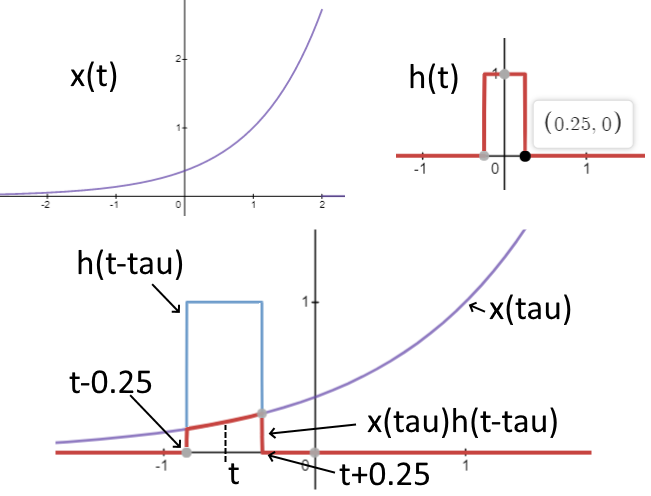
\includegraphics[width=0.8\linewidth]{q2d}
\end{center}

For $-\infty < t \leq 1.75$:
\begin{align*}
	y(t) &= \int_{t-0.25}^{t+0.25} e^{\tau-1}\di\tau \\
	&= \Eval{e^{\tau-1}}{t-0.25}{t+0.25} \\
	&\approx 0.186e^t.
\end{align*}

For $1.75 < t \leq 2.25$:
\begin{align*}
	y(t) &= \int_{t-0.25}^{2} e^{\tau - 1}\di\tau \\
	&= \Eval{e^{\tau-1}}{t-0.25}{2} \\
	&= e-e^{t-1.25}.
\end{align*}

For $t > 2.25$, $y(t) = 0$.

$\bullet$ \textit{Given $x(t)$ below, find any symmetry exhibited and find the trigonometric Fourier series coefficients of $x(t)$.}
\begin{center}
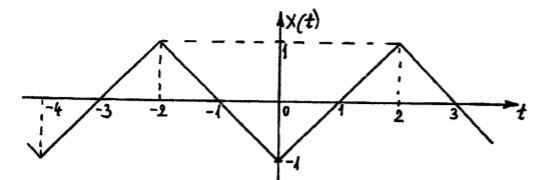
\includegraphics[width=0.8\linewidth]{q3a}
\end{center}

$x(t)$ exhibits even symmetry and half-wave odd symmetry. This means that $b_n = 0$ for all $n$ and $a_n = 0$ for even $n$ (and hence, $a_0 = 0$). Due to even symmetry, we have
\[ a_n = \dfrac{4}{T} \int_{0}^{T/2} x(t)\cos\pfrac{2\pi nt}{T} \di t. \]
Note that $x(t)$ can be written as
\[ x(t) = t - 1 \quad \text{for $0 \leq t \leq 2$.} \]
So, since the period of $x(t)$ is $T = 4$,
\begin{align*} 
	a_n &= \dfrac{4}{4} \int_0^2 (t-1)\cos\pfrac{\pi n t}{2} \di t \\
	&= \int_0^2 t\cos\pfrac{\pi n t}{2}\di t - \int_0^2 \cos\pfrac{\pi n t}{2}\di t \\
	&= \dfrac{2}{n\pi} \int_0^2 \dfrac{\pi n t}{2}\cos\pfrac{\pi n t}{2}\di t - \Eval{\dfrac{\sin\pfrac{\pi n t}{2}}{\frac{\pi n}{2}}}{0}{2} \\
	& \rightarrow \text{let } x = \frac{\pi nt}{2} \\
	&= \pfrac{2}{n\pi}^2\int_{0}^{n\pi}x\cos x \di x - \underbrace{\bracks{ \dfrac{\sin(n\pi)}{\frac{n\pi}{2}} - 0 }}_{=0} \\
	&= \pfrac{2}{n\pi}^2 \Eval{\bracks{ \cos x + x\sin x }}{0}{n\pi} \\
	&= \pfrac{2}{n\pi}^2 \bracks{\cos(n\pi) - 1} \\
	&= \begin{cases}
		-2\pfrac{2}{n\pi}^2, n \text{ odd}, \\
		0, n \text{ even}.
	\end{cases}
\end{align*}

\underlineSection[Miscellaneous Identities]
\[ \sin(t) = \dfrac{1}{2j}\bracks{ e^{jt}-e^{-jt} } \]
\[ \cos(t) = \dfrac{1}{2}\bracks{ e^{jt}+e^{-jt} } \]

\end{multicols*}


\end{document}
